
% Inbuilt themes in beamer
\documentclass{beamer}

% Theme choice:
\usetheme{Warsaw}

% Title page details: 
\title{Strategic Patient Discharge:\\ The Case of Long-Term Care Hospitals} 
\subtitle{Paul J. Eliason\\ Paul L. E. Grieco\\ Ryan C. McDevitt\\ James W. Roberts\\ \textit{American Economic Review 2018}}
\author{Presented by: Ka Yan CHENG}
\date{ \vspace*{-1cm}\\ ECON 771 Health Economics II, Fall 2022}

% Fix the footline too long problem
\setbeamertemplate{headline}{}
\setbeamertemplate{footline}{%
  \leavevmode%
  \hbox{\begin{beamercolorbox}[wd=.5\paperwidth,ht=4.5ex,dp=2.125ex,leftskip=.3cm plus1fill,rightskip=.3cm]{author in head/foot}%
    \usebeamerfont{author in head/foot}\insertshortauthor
  \end{beamercolorbox}%
  \begin{beamercolorbox}[wd=.5\paperwidth,ht=4.5ex,dp=2.125ex,leftskip=.3cm,rightskip=.3cm plus1fil]{title in head/foot}%
    \usebeamerfont{title in head/foot}
    \parbox{.45\paperwidth}{\inserttitle}
  \end{beamercolorbox}}%
  \vskip0pt%
}

% Change subtitle format
\setbeamercolor{subtitle}{fg=lightgray}%
\setbeamerfont{subtitle}{size=\scriptsize}%



\setbeamerfont{date}{size=\footnotesize}


\begin{document}

% Title page frame
\begin{frame}
    \titlepage 
\end{frame}

% Remove logo from the next slides
\logo{}


% Outline frame
\begin{frame}{Outline}
    \tableofcontents
\end{frame}


% Lists frame
\section{Motivation}

\begin{frame}{Motivation}
\framesubtitle{"The Magic Day" - Short-stay outliers (SSOs) threshold}
Reform of the Prospective Payment System(PPS) Medicare system
\begin{itemize}
	\item Before 2002 -- \\
			\begin{itemize}
				\item Medicare pay LTCHs a fixed 5\% mark-up over reported cost ("Cost-plus")
				\end{itemize}
	\item Since 2002 -- \\
			\begin{itemize}
			\item \textbf{SSOs threshold} (five-sixths of the geometric mean of the length of stay for each DRG) introduced to discourage needless transfer from general acute-care hospitals to LTCHs
			\item SSOs case are paid linearly with the length of stay and the payment is much smaller
			\end{itemize}
\end{itemize}


\end{frame}


\begin{frame}{Motivation}
\framesubtitle{"The Magic Day" - Short-stay outliers (SSOs) threshold}
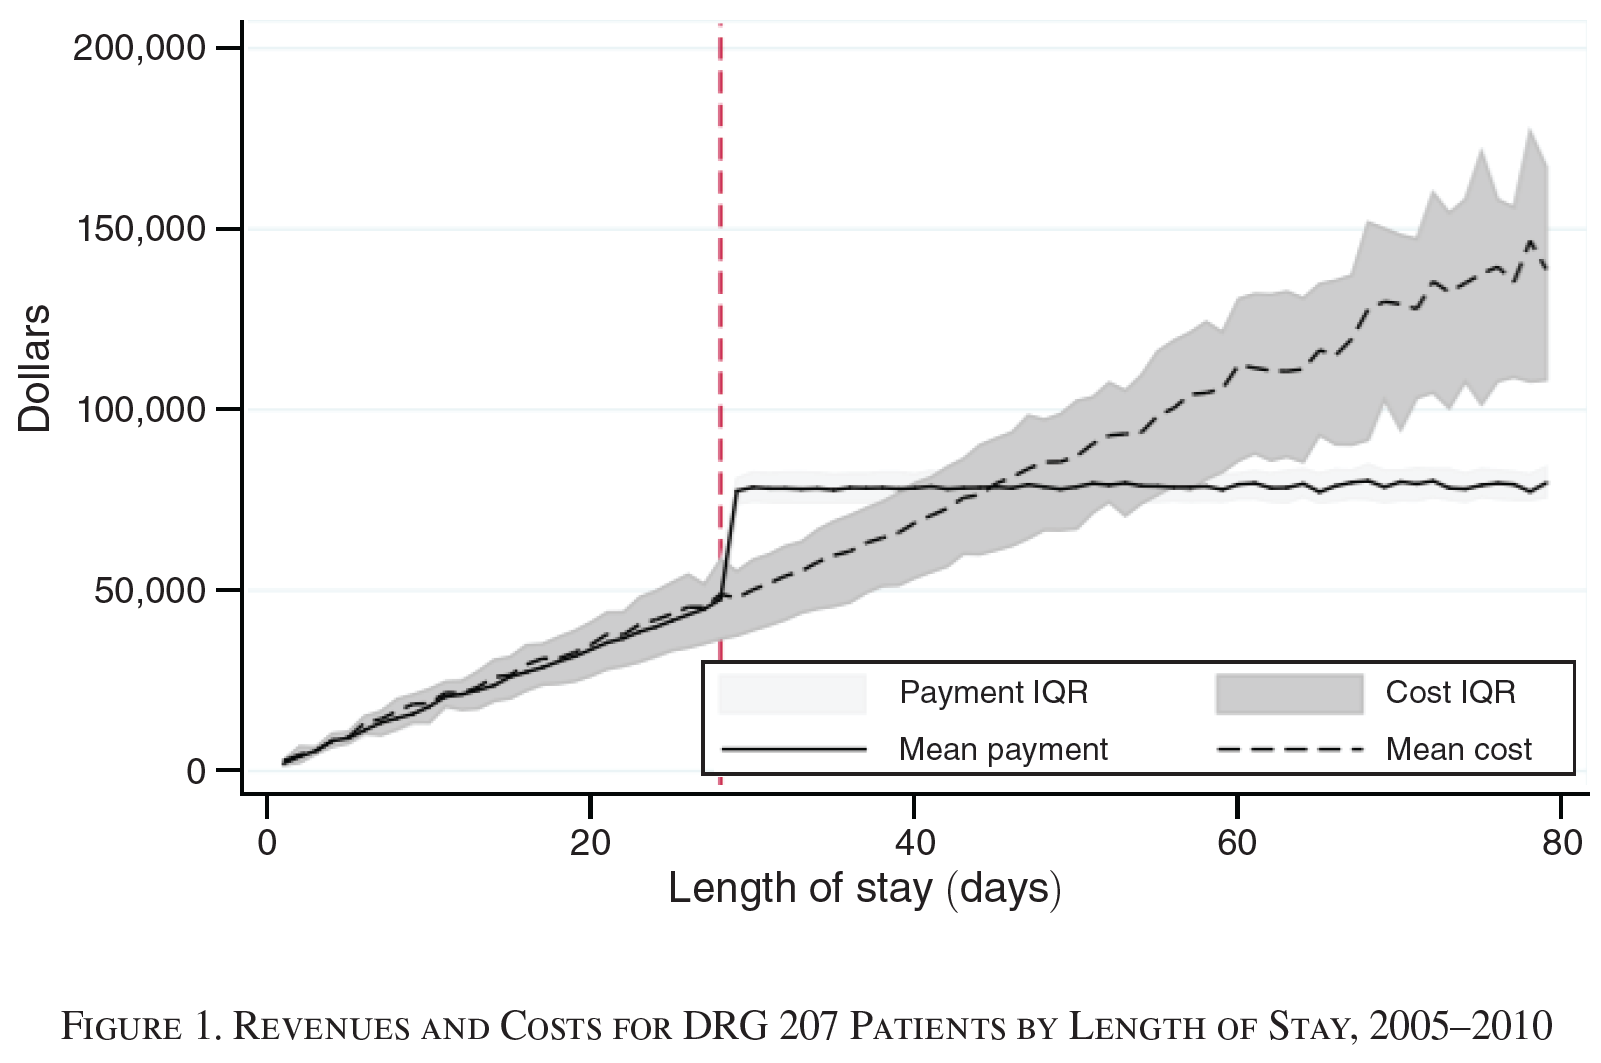
\includegraphics[width=\textwidth]{Rev_Cost_DRG207}

\end{frame}

%Reseach question
\section{Research question}
\begin{frame}{Research question}
\begin{enumerate}
    \item \color<2->{lightgray} Given the financial incentives, \textbf{do LTCHs demonstrate strategic discharge} and \textbf{how is the SSO threshold effect}?
		$\Rightarrow$ Graphical evidence and Probit regression models
	
    \item<2-> \color<2->{black} \textbf{How LTCHs would behave under alternative payment schemes?}
		 \begin{enumerate}
		\item Hospital payments independent of a patient's length of stay
		\item New proposal by MedPAC -- \\ The "per diem counterfactual"
		\item Policy prior to having PPS for LTCHs -- \\ The cost-plus reimbursement scheme
		\end{enumerate}
		$\Rightarrow$ Dynamic structural model
\end{enumerate}
\end{frame}

%Contribution
\section{Contribution}
\begin{frame}{Contribution}
On the topic of agents' responses to incentives to reduce health care expenditures: \textbf{Inpatient hospitals} 

\end{frame}

%Preview of findings
\section{Preview of findings}
\begin{frame}{Preview of findings}
		 \begin{enumerate}
		\item The SSO threshold effect
				 \begin{itemize}
				\item LTCHs respond to the financial incentives by holding patients until right after
they reach this point
				\end{itemize}
		\item Alternative payment systems that remove the sharp jump would provide substantial savings for Medicare.
		\end{enumerate}
\end{frame}

%Data
\section{Data}
\begin{frame}{Data}
\begin{enumerate}
\item Claims dataset from CMS
		\begin{itemize}
		\item cover all Medicare beneficiaries stays at LTCHs
		\item 2002 (old reimbursement system) and 2004-2013
		\item DRG/Medicare payments/Covered costs/Length of stay/Diagnosis and procedural
codes/Race/Age/Gender/Type of hospital admission/Patient was discharged alive?/If alive, the discharge destination
		\end{itemize}
\item Data on hospital characteristics from CMS and the American Hospital Association (AHA)
		\begin{itemize}
		\item Name/Location/Hospital type/Size/For-profit status/Medical
			school affiliation/Services offered/\color{teal}Hospital's CMS certification number
		\end{itemize}
\end{enumerate}
\end{frame}

\section{The SSO Threshold Effect}
\begin{frame}{The SSO Threshold Effect - DRG 207}
\framesubtitle{Graphical Evidence - DRG 207}
\begin{center}
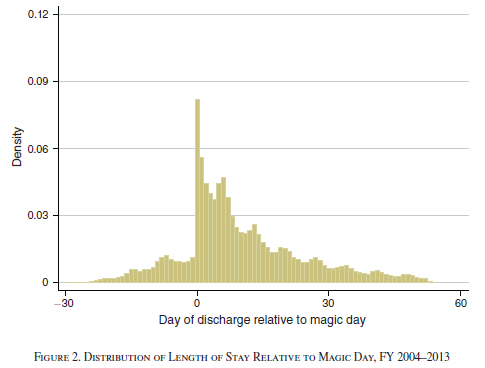
\includegraphics[height=6cm]{graph_evi_grouped}
\end{center}
Qs: What if the SSO threshold really reflects the clincal nature of the DRG?
\end{frame}

\begin{frame}{The SSO Threshold Effect}
\framesubtitle{Graphical Evidence - By Year}
\begin{center}
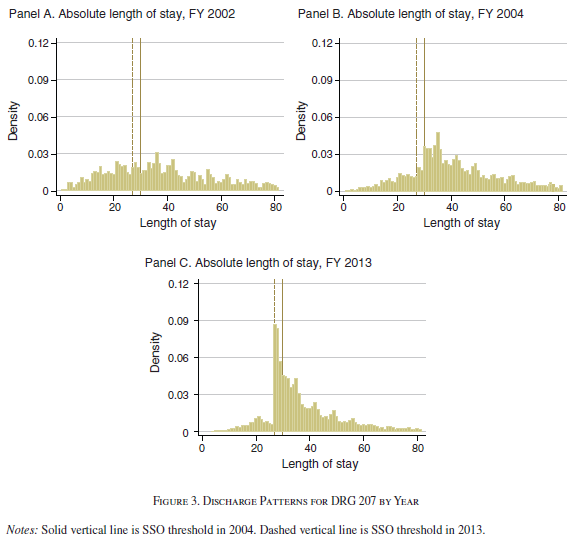
\includegraphics[height=8cm]{graph_evi_across_time}
\end{center}
\end{frame}

\begin{frame}{The SSO Threshold Effect}
\framesubtitle{Graphical Evidence - By Destination}
\begin{center}
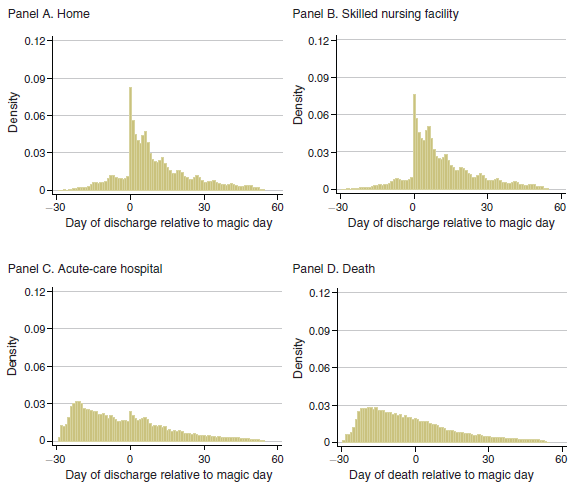
\includegraphics[height=7cm]{graph_evi_dest}
\end{center}
\end{frame}

\begin{frame}{The SSO Threshold Effect}
\framesubtitle{Graphical Evidence - By LTCH Location Type}
\begin{center}
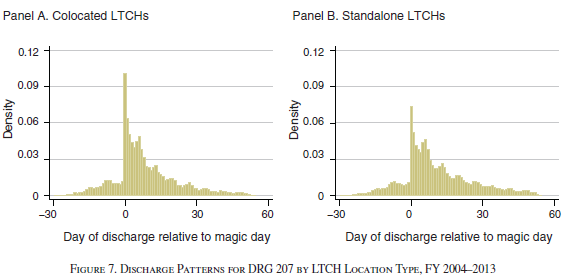
\includegraphics[height=5cm]{graph_evi_loc}
\end{center}
\end{frame}

\begin{frame}{The SSO Threshold Effect}
\framesubtitle{Graphical Evidence - By LTCH Profit Type}
\begin{center}
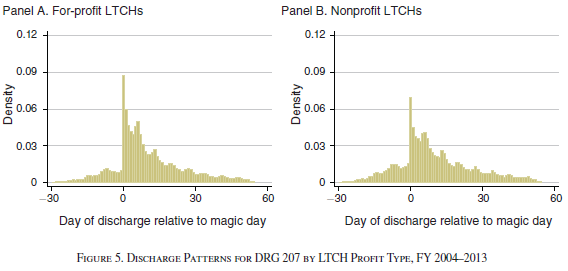
\includegraphics[height=5cm]{graph_evi_prof}
\end{center}
\end{frame}

\begin{frame}{The SSO Threshold Effect}
\framesubtitle{Quantifying the Effect - Probit models}
\begin{equation}
\text{Pr}(discharge|t,s) = \Phi( \gamma_0 + \gamma_1 t + \gamma_2 t^2 + \mu_s )
\end{equation}
$t$: Absolute day of hospital stay, $s$: day relative to the threshold
*Note: $s$ is not a function of $t$ [SSO threshold changes over time]
\begin{center}
\includegraphics[height=5cm]{probit_result}
\end{center}
\end{frame}

\begin{frame}{The SSO Threshold Effect}
\framesubtitle{Quantifying the Effect - Probit models}
\begin{equation}
\text{Pr}(discharge|t,s) = \Phi( \gamma_0 + \gamma_1 t + \gamma_2 t^2 + \mu_{s, \color{red}x(i)})
\end{equation}
\begin{center}
\includegraphics[height=3cm]{probit_result_bygroup}
\end{center}
\end{frame}

\section{Counterfactual Analysis}
\begin{frame}{Counterfactual Analysis}
\framesubtitle{The Dynamic Structural Model - Set Up}
Idea: Model daily decision of an LTCH to discharge a patient\\

\begin{equation}
u_t = \lambda_t + \alpha p_t
\end{equation}
\begin{equation*}
p_t = \begin{cases}
p&\text{for $t < t^m$}\\
P - (t^m - 1) \times p &\text{for $t = t^m$} \\
0 &\text{for $t > t^m$}
\end{cases}
\end{equation*}
Bellman equation:
\begin{equation}
V_t(\varepsilon_t) = u_t + \text{max\{$\varepsilon_{kt} + \delta EV_{t+1} + \varepsilon_{dt} $\}}
\end{equation}
\end{frame}

\begin{frame}{Counterfactual Analysis}
\framesubtitle{The Dynamic Structural Model - Estimation }
\begin{enumerate}
	\item Payment policies
			\begin{equation}
			V_t(\varepsilon_t) = u_t + \text{max\{$\varepsilon_{kt} + \delta EV_{t+1} + 				\varepsilon_{dt} $\}}
			\end{equation}
	\item Non-revenue benefits ($\lambda_t$)
			\begin{equation}
		\lambda_{i,t} = \gamma_{0, DRG} + \gamma_{1, DRG}t+ \gamma_{2, DRG}t^2+ \gamma_{3, DRG}t^3 - \beta \hat{c_h} + \Psi_{day of week}
			\end{equation}
	\item \textbf{KEY} parameter of interest: Effect of payment structure on discharge decision
			\begin{equation}
			\alpha = \alpha_k + \alpha_z
			\end{equation}
\end{enumerate}
\end{frame}

\begin{frame}{Counterfactual Analysis}
\framesubtitle{Simulating Alternative Payment Schemes - Estimation}
\begin{center}
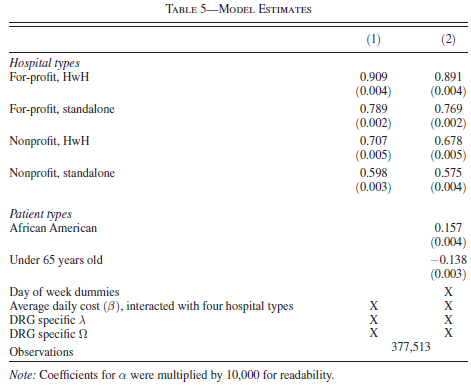
\includegraphics[height=6cm]{dyn_est}
\end{center}
\end{frame}

\begin{frame}{Counterfactual Analysis}
\framesubtitle{Simulating Alternative Payment Schemes - Discharge probabilities}
\begin{center}
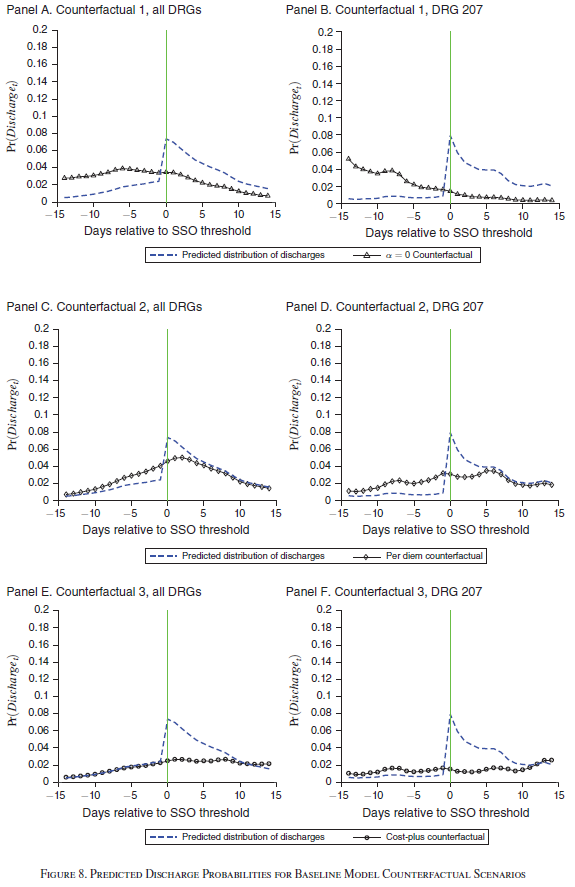
\includegraphics[height=8cm]{counter_discharge_prob}
\end{center}
\end{frame}

\begin{frame}{Counterfactual Analysis}
\framesubtitle{Simulating Alternative Payment Schemes - Outcomes}
\begin{center}
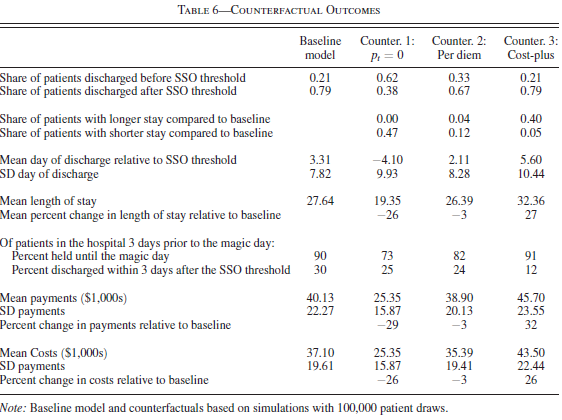
\includegraphics[height=6cm]{counter_outcome}
\end{center}
\end{frame}

%Threats
\section{Threats}
\begin{frame}{Threats}
\begin{itemize}
\item Estimation on the dynamic structural model is just based on data of the 9 most common DRGs, is it general enough to make a conclusion? 
\item Maybe under alternative payment systems, hospitals behave differently when treating less common DRGs? 
\end{itemize}
\end{frame}

%Results
\section{Conclusion}
\begin{frame}{Conclusion}
Sharp jump in the LTCH Medicare payment system induced strategic discharge that based on financial incentives outside of clinical consideration, aternative proposal that remove the jump can bring substantial saving to Medicare (at least when paying for some of the DRGs).
\end{frame}

\end{document}